\section{Description et conception des états}

\subsection{Description des états}

Le diagramme des états possède pour l'instant 18 classes. Tous les attributs présentés seront private sauf si précisé autrement.

\subsubsection{Etat du jeu}

\underline{\textbf{InfoPlayer}}
\par Cette classe contient les informations d'initialisations d'un joueur. Elle est utilisée pour initialiser le joueur, son deck, et également la map créée.

\begin{itemize}
        \item int firstElement : élément de départ du joueur. Les valeurs autorisées sont 1 (Air), 2 (Water), 3 (Earth), 4 (Fire). La valeur par défaut est 1. 
        \item  bool playerControlledByAI : indique si le joueur est controlé par une intelligence artificielle ou non.
\end{itemize}

\underline{\textbf{Rules}}
\par Cette classe contient les informations du/des joueur(s) et si le jeu est fini ou non.
\begin{itemize}
    \item bool isGameLost : Indique si les joueurs ont gagné ou non. Implique que le jeu est terminé. Le jeu est perdu lorsque que tous les joueurs sont morts.
    \item bool isGameOver : Indique si le jeu est terminé ou non. Un jeu est terminé lorsqu'il est perdu, ou lorsque les joueurs ont traversé la dernière salle du dernier étage.
    \item int nbPlayers : indique le nombre de joueurs qui participeront au jeu. Les valeurs autorisées sont 1 ou 2. Ces joueurs joueront en coopératif et affronteront les ennemis ensemble.
    \item  std::vector<std::unique\_ptr<InfoPlayer>> infoPlayer: vecteur de pointeurs vers un objet InfoPlayer. Contient les informations du joueur 1 et 2 (s'il existe) respectivement. sa taille maximale est de 2, sa taille minimale est de 1.
\end{itemize}

\underline{\textbf{GameState}}
\par Contient des pointeurs vers tous les objets du jeu.
\begin{itemize}
    \item std::vector<Player*> players : Un vecteur de pointeurs vers les joueurs. Sa taille minimale est de 1, sa taille maximale est de 2.
    \item std::unique\_ptr<Map> map: Un pointeur vers la carte du jeu. La carte est composée d'étages (Floor), eux-même composés de salles (Room). 
    \item std::unique\_ptr<Rules> rules : un pointeur vers un objet Rules qui défini les règles du jeu.
    \item  bool isInsideRoom : Indique si les joueurs se trouvent dans une salle ou  à l'exterieur. S'ils se trouvent à l'extérieur, c'est qu'ils sont en train de choisir une salle. Ils ont alors vue sur l'ensemble du graph des salles. Sinon, ils se trouvent à l'intérieur et effectuent les actions correspondantes. Les deux joueurs sont toujours en même temps à l'intérieur ou à l'exterieur d'une salle.
\end{itemize}

\subsubsection{Etat de la carte}
\underline{\textbf{Map}}
\par Contient des pointeurs vers les différentes étages.
\begin{itemize}
    \item std::vector<std::share\_ptr<Floor>> floors: vercteur de pointeurs vers les différents étages (Floor). Il y a forcément 4 étages (un pour chaque élément), donc ce vecteur est de taille 4. 
    \item int currentFloor : la référence vers l'étage actuel. Forcément comprise entre 0 et 3 inclus.
\end{itemize}

\underline{\textbf{Floor}}
\par Contient des pointeurs vers les différentes salles. Les salles sont organisées à l'aide d'un graphe orienté. 
\begin{itemize}
    \item int floorNumber : le numéro de l'étage. Compris entre 0 et 3 inclus. En plus de référencer l'étage, ce nombre est utilisé pour instancier les salles et les monstres afin d'avoir une difficulté graduée.
    \item std::shared\_ptr<Room> currentRoom : un pointeur vers la salle à laquelle se situent les joueurs.
    \item int element : indique l'élément de l'étage. Les valeurs autorisées sont 1 (Air), 2 (Water), 3 (Earth), 4 (Fire). Sert à instancier la majorité des ennemis de cet étage avec cet élément.
    \item std::string floorImage : chaîne de caractère qui indique le chemin vers l'image associée à l'étage. Ce chemin doit référencer une image du dossier du projet. Il y a une image différente pour chaque étage.
    \item std::shared\_ptr<Room> firstRoom : un pointeur vers la première salle du graphe orienté. Cette salle est unique et sera considérée comme l'origine du graphe. Aucune salle ne pointe vers elle.
    
\end{itemize}

\underline{\textbf{Room}}
\par Il existe 3 types de salle: les salles d'ennemis (EnemyRoom), les salles de repos (SleepRoom) et les salles spéciales (SpecialTrainingRoom).
\begin{itemize}
    \item int element : l'élement de la salle (Room). Les valeurs autorisées sont 1, 2, 3 ou 4 pour chacun des éléments. Une salle peut être d'un élément différent que celui de l'étage dont elle fait partie.
    \item std::string imageMapRoom : chaîne de caractères qui indique le chemin vers l'image associée à la salle. Ce chemin doit référencer une image du dossier du projet. Cette image sera utilisée pour l'affichage de la salle sur la carte (lorsque les joueurs seront en dehors de la salle).
    \item std::string imageInsideRoom : chaîne de caractères qui indique le chemin vers l'image associée à la salle. Ce chemin doit référencer une image du dossier du projet. Cette image sera utilisée lors de l'affichage de l'intérieur de la salle (lorsque les joueurs seront dans la salle).
    \item bool isSpecialTrainingRoom : un booléen indiquant si la salle est une salle spéciale (true) ou non (false). Doit être false si au moins un parmi isEnemyRoom ou isSleepRoom est true.
    \item bool isEnemyRoom : un booléen indiquant si la salle est une salle d'ennemis (true) ou non (false). Doit être false si au moins un parmi isSpecialTrainingRoom ou isSleepRoom est true.
    \item bool isSleepRoom : un booléen indiquant si la salle est une salle de repos (true) ou non (false). Doit être false si au moins un parmi isEnemyRoom ou isSpecialTrainingRoom est true.
    \item std::shared\_ptr<Room> nextRoom : pointeur vers la salle suivante dans le graphe. Il n'y a pour l'instant qu'un unique chemin pour le graphe orienté.
\end{itemize}

\underline{SpecialTrainingRoom}
\par Hérite de la classe Room. Permet aux joueurs d'ajouter des cartes à son deck.
\begin{itemize}
    \item std::vector<Card*> cardReward : un vecteur de pointeurs vers des cartes. La taille de ce vecteurs est 3. Les cartes peuvent être générées avec n'importe quel élément.
\end{itemize}

\underline{SleepRoom}
\par Hérite de la classe Room. Permet aux joueurs de se reposer et de regagner de la vie.
\begin{itemize}
    \item int heal : indique la valeur de vie que récupèrera un joueur en se reposant. Valeur positive requise.
\end{itemize}

\underline{EnemyRoom}
\par Hérite de la classe Room. Les joueurs doivent affronter un ou plusieurs ennemis et les vaincre pour pouvoir passer à la salle suivante.
\begin{itemize}
    \item std::vector<std::unique\_ptr<Enemy>> enemies : un vecteur de pointeurs vers des objets de classe Enemy. Ce vecteur possède une taille minime de 1 et maximale de 3.
    \item std::vector<std::unique\_ptr<DeckParts>> drawPiles : un vecteur de pointeurs vers des objets de type DeckParts. Le vecteur possède une taille minimale de 1 et maximale de 2. Référence la pioche (drawPile) de chacun des joueurs.
    \item std::vector<std::unique\_ptr<DeckParts>> hands : un vecteur de pointeurs vers des objets de type DeckParts. Le vecteur possède une taille minimale de 1 et maximale de 2. Référence la main (hand) de chacun des joueurs. Une seule main sera affichée à la fois.
    \item std::vector<std::unique\_ptr<DeckParts>> discardPiles: un vecteur de pointeurs vers des objets de type DeckParts. Le vecteur possède une taille minimale de 1 et maximale de 2. Référence la défausse (discardPile) de chacun des joueurs.
    \item int turn : nombre de tours écoulés depuis le début du combat. Valeur positive requise. 
    \item int entityTurn : indique l'identifiant (Id) de l'entité en train de jouer. Si cet identifiant correspond à un joueur, sa main sera affichée et il pourra jouer des cartes. Si cet Id correspond à un ennemi, il effectuera son action puis choisira sa suivante en fonction des actions précédentes des joueurs.
    \item bool isGameLost : indique si les joueurs ont perdu. Le combat continue tant que les joueurs n'ont pas gagné, perdu ou abandonné. Les joueurs gagnent ce combat s'ils réduisent à 0 la vie des monstres adverses, perdent si leur vie est réduite à 0 ou s'ils abandonnent. Si les joueurs gagnent, ils sortent de la salle.
    
\end{itemize}


\subsubsection{Etat du deck}
\underline{\textbf{Card}}
\par Définie les cartes jouées dans le jeu.
\begin{itemize}
    \item std::string name : le nom de la carte. Doit être un nom de carte existant.
    \item int cost : le coût en énergie de la carte. Les valeurs possibles sont comprises entre 0 et 3 inclus. 
    \item int target : indique à quel type d'entité s'applique la carte. Les valeurs possibles sont 0 (unique joueur), 1 (unique ennemi), 2 (tous les ennemis), 3 (tous les joueurs).
    \item std::string image : chemin vers l'image de la carte. Cette image doit appartenir au dossier.
    \item int element : l'élément de la carte. Les valeurs possibles sont 0 (None), 1 (Air), 2 (Water), 3 (Earth), 4 (Fire). 
    \item int attack : valeur d'attaque de la carte. Indique le nombre de points de vie perdus par la cible lorsque la carte est jouée (hors bonus ou malus du joueur). Valeur positive requise.
    \item int block : valeur de block de la carte. Indique le nombre de block gagné par la cible losque la carte est jouée (hors bonus ou malus du joueur). Valeur positive requise. 
    \item int draw : indique le nombre de cartes piochées lorsque cette carte est jouée. Les cartes piochées passent de la pile de pioche à la main. Si la main est pleine, on ne pioche pas davantage. Valeur positive requise.
    \item int discard : indique le nombre de cartes défaussées lorsque cette carte est jouée. Les cartes défaussées vont de la main à la défausse. Valeur positive requise.
    \item int heal : valeur de soin de la carte. Soigne la cible du montant indiqué lorsque la carte est jouée. Valeur positive requise. Principe différent de l'attribut "heal" de la classe Buff.
    \item Debuff debuff : objet Debuff contenant des malus à appliquer aux cartes au moment où elles sont jouées.
    \item Buff buff : objet Buff contenant des bonus à appliquer aux cartes au moment où elles sont jouées.
\end{itemize}

\underline{\textbf{CardManager}}
\par Singleton permettant de créer les cartes de façon unique, puis d'y avoir accès facilement et enfin de les détruire facilement.
\begin{itemize}
    \item static CardManager* inst : Unique instance du CardManager
    \item std::vector<std::unique\_ptr<Card>> cards : Vecteur de cartes
\end{itemize}

\underline{\textbf{Deck}}
\par Contient des pointeurs vers des cartes. 
\begin{itemize}
    \item std::vector<Card*> cards : contient un vecteur de pointeurs vers des cartes. Certains pointeurs peuvent pointer vers la même carte. Ce vecteur possède une taille positive (par défaut 15) égale à sizeMax.
    \item int size : la taille du sous-vecteur à considérer. Si un deck est incomplet ou que des cartes ont été retirées, on ignore simplement les pointeurs correspondant et on considère un vecteur de taille plus petite. Valeur positive nécessaire.
    \item int sizeMax : la taille maximale du deck autorisée. Valeur positive nécessaire. Par défaut 15.
\end{itemize}

\underline{\textbf{DeckParts}}
\par Permet de créer la pioche, la main et la défausse pour une salle d'ennemis.

\begin{itemize}
    \item std::vector<Card*> cards : un vecteur de pointeurs vers des cartes. Certains pointeurs peuvent pointer vers la même carte. Possède une taille positive, égale à sizeMax.
    \item Player* player: pointeur vers le joueur auquel la pioche/main/défausse appartient.
    \item bool isHand : indique si la partie de deck est une main ou non. Une partie de deck ne peut être qu'une seule de ces instances: pioche, main, défausse.
    \item bool isDiscardPile: indique si la partie de deck est une défausse ou non. Une partie de deck ne peut être qu'une seule de ces instances: pioche, main, défausse.
    \item bool isDrawPile : indique si la partie de deck est une pioche ou non. Une partie de deck ne peut être qu'une seule de ces instances: pioche, main, défausse.
    \item int size : la taille du sous-vecteur à considérer. Valeur positive requise.
    \item int sizeMax : taille maximale du vecteur de cartes (cards) possible. Valeur positive requise.
\end{itemize}

\underline{\textbf{Buff}}
\par Contient les buffs à appliquer à une entité lorsqu'elle attaque ou à chacun de ses tours.
\begin{itemize}
    \item int blockPlus : Valeur positive requise. Augmente le nombre de block réalisé de toute carte jouée de 50\% pendant le nombre de tour indiqué par blockPlus. blockPlus diminue à chaque début du tour du joueur.
    \item int attackPlus : Valeur positive requise. Augmente  l'attaque réalisée de toute carte jouée de 50\% pendant le nombre de tour indiqué par attackPlus. attackPlus diminue à chaque début du tour du joueur.
    \item int heal : Valeur positive requise. Soigne le joueur à la fin de son tour de la valeur indiquée par heal. Cette valeur décrémente à chaque début de tour. (Pour heal = 4, le joueur se soigne de 4 au tour n, puis de 3 au tour n+1, etc).
    \item int evade : Valeur positive requise. Esquive un nombre d'attaque indiqué par evade. Les attaques esquivées ne sont pas choisiées, ce sont les prochaines attaques lancées par le monstre. Elles sont esquivées même si la valeur du block était suffisante pour parer entièrement l'attaque.
    \item int retaliate : Valeur positive requise. Inflige 5 points de dégats par attaque reçue à l'attaquant. S'applique pendant les actions de l'ennemi, pendant le nombre de tour indiqué par retaliate. Cette valeur diminue au début du tour du joueur.
\end{itemize}

\underline{\textbf{Debuff}}
\par Contient les debuffs à appliquer à une entité lorsqu'elle attaque ou à chacun de ses tours.
\begin{itemize}
    \item int blockMinus: Valeur positive requise. Diminue la valeur de block réalisée de toute carte jouée de 50\% pendant le nombre de tour indiqué par blockMinus. blockMinus diminue à chaque début du tour du joueur.
    \item int attackMinus: Valeur positive requise. Diminue la valeur d'attaque réalisée de toute carte jouée de 50\% pendant le nombre de tour indiqué par attackMinus. attackMinus diminue à chaque début du tour du joueur.
\end{itemize}

\subsubsection{Etat des entités}
\underline{\textbf{Entity}}
\par Contient les informations principales d'une entité. Ses identifiants, sa vie... Se décompose en joueur (Player) ou ennemi (Enemy).
\begin{itemize}
    \item std::string name : nom de l'entité. S'il s'agit d'un ennemi, ce nom doit référencer un nom d'ennemi existant. 
    \item int id : identifiant de l'entité. Valeur positive requise. Deux entités ne peuvent pas posséder le même identifiant, même si par exemple se sont deux ennemis possèdant les même caractéristiques. Les identifiants des joueurs seront 0 ou 1, ceux des monstres auront des valeurs supérieures strictement à 1.
    \item int life : la vie d'une entité. Valeur positive nécéssaire. Une entité perd de la vie si elle reçoit des attaques alors qu'elle n'a pas suffisemment de block. Si la vie d'une entité passe à 0 elle est considérée comme morte.
    \item int element : element de l'entité. Valeurs possibles: 0 (None), 1 (Air), 2 (Water), 3 (Earth), 4 (Fire). Ces valeurs changeront en fonction des cartes jouées (pour les joueur seulement).
    \item std::string image : chemin vers l'image utilisée lors de l'affichage de l'entité. Ce chemin doit référencer une image existante du dossier.
    \item int statAttack : stat de base de l'attaque. Valeur positive requise. La statAttack s'additionne à l'attribut attack d'une carte (pour les joueurs) ou d'un skill (pour les ennemis) pour le calcul final des dégats causés à la cible. La statAttack de base des ennemis est fixée en fonction du numéro de l'étage  et de la salle actuels.
    \item int statBlock : stat de base du block. Valeur positive requise. La statBlock s'additionne à l'attribut attack d'une carte (pour les joueurs) ou d'un skill (pour les ennemis) pour le calcul final du block obtenu par la cible.  La statBlock de base des ennemis est fixée en fonction du numéro de l'étage et de la salle actuels.
    \item int block : la valeur de block. Valeur positive requise. Le block permet de parer des attaques. Au lieu de perdre des points de vie, une entité perd de son block. Elle perd le reste des points de vie si son block passe à 0. Le bloc est initialisé à 0 au début de chaque tour d'une entité.
    \item Buff buff : les buffs appliqués à l'entité.
    \item Debuff debuff : les debuffs appliqués à l'entité.
    \item bool isPlayer : indique si l'entité est un joueur (true) ou un ennemi (false).
    \item bool isEntityAlive : indique si l'entité est en vie. Une entité n'est pas en vie si son total de vie est nul. Une entité n'est pas affichée si elle n'est pas en vie, et ne peut plus agir pour le reste du jeu/combat. Si aucun des joueurs n'est en vie, la partie est terminée.
    \item int maxLife : la valeur maximale de la vie de cette entité.
\end{itemize}


\underline{\textbf{Enemy}}
\par Hérite de Entity. Une classe pour les ennemis. 
\begin{itemize}
    \item std::vector<Card*> reward : un vecteur de pointeurs vers les cartes. Ce vecteur est de taille 3. Les cartes pointées peuvent être ajoutées au deck d'un joueur lorsque le combat est terminé. Un joueur ne pourra ajouter qu'une seule carte parmis toutes les cartes proposées (même s'il y a eu plusieurs ennemis).
    \item std::vector<EnemySkill*>  skills : un vecteur de pointeurs vers les capacités (Skill) d'un ennemi. Ce vecteur possède une taille minimale de 1 et maximale de 10. Détermine les capacités pouvant être effectuées par un ennemi.
    \item int intent : un entier. Fait référence au pointeur de la capacité qui va être utilisée par l'ennemi lors de son tour. Valeur comprise entre 0 et la taille de skills - 1, soit au moins comprise entre 0 et 10. 
\end{itemize}

\underline{\textbf{EnemySkill}}
\par Capacité des ennemis. Semblable aux cartes pour les attributs.

\begin{itemize}
    \item int attack : Valeur d'attaque de la capacité (buffs/debuffs non appliqués). Valeur positive requise.
    \item int block : Valeur de block de la capacité (buffs/debuffs non appliqués). Valeur positive requise.
    \item int heal : Valeur de soin de la capacité. Valeur positive requise.
    \item std::unique\_ptr<Buff>  buff : bonus que la capacité va appliquer sur la cible. Ils vont s'additionner à ses bonus actuels.
    \item std::unique\_ptr debuff : malus que la capacité va appliquer sur la cible. Ils vont s'additionner à ses malus actuels.
    \item std::string intentImage : chemin vers l'image de référence de l'attaque. Cette image apparaitera au dessus de l'ennemi en combat et indiquera au joueur le type de capacité utilisée. Ces images sont de deux catégories: celles représentant une capacité menée sur un joueur(ou tous les joueurs) et celles menées sur un ennemi (ou tous les ennemis).
    Capacités sur les joueurs : attaque, attaque et debuff.
    Capacités sur les ennemis : bloque, buff, soigne et toutes les combinaisons de ces paramètres. On a au total 9 images différentes pour les images d'intention.
    \item int cooldown : Valeur positive requise. Un entier qui indique le nombre minimum de tours requis avant de pouvoir réutiliser cette capacité. 
    \item int turnsBeforUse : Valeur positive requise. Un entier qui indique le nombre de tours restant avant de pouvoir réutiliser cette capacité. Après l'utilisation de la capacité, turnsBeforeUse prend la valeur cooldown, puis est décrémentée à chaque tour jusqu'à atteindre 0.
    \item int target: indique à quel type d'entité s'applique la capacité. Les valeurs possibles sont 0 (unique joueur), 1 (unique ennemi), 2 (tous les ennemis), 3 (tous les joueurs).
\end{itemize}

\underline{\textbf{SkillManager}}
\par Singleton permettant de créer les compétences des enemis de façon unique, puis d'y avoir accès facilement et enfin de les détruire facilement.
\begin{itemize}
    \item static SkillManager* inst : Unique instance du SkillManager
    \item std::vector<std::unique\_ptr<EnemySkill>> cards : Vecteur de competences.
\end{itemize}

\underline{\textbf{Player}}
\par Hérite de la classe Entity. Contient les informations relatives au joueur.
\begin{itemize}
    \item int energy : valeur positive requise. Le nombre d'énergie restante du joueur. Cette énergie est utilisée pour jouer des cartes, une carte ne peut pas être jouée si son coût est supérieur à l'énergie du joueur. L'énergie est initialisée à 3 au début de chaque tour du joueur.
    \item std::unique\_ptr<Deck>  deck : un pointeur vers un deck de cartes.
\end{itemize}

\underline{\textbf{PlayerManager}}
\par Singleton permettant de créer les personnages des joueurs de façon unique, puis d'y avoir accès facilement et enfin de les détruire facilement.
\begin{itemize}
    \item static PlayerManager* inst : Unique instance du PlayerManager
    \item std::vector<std::unique\_ptr<Player> > cards : Vecteur de joueurs
\end{itemize}

\subsection{Conception Logiciel}

Les figures qui suivent présentent notre diagramme de classe sous forme de diagramme UML.


\begin{landscape}
\begin{figure}[p]
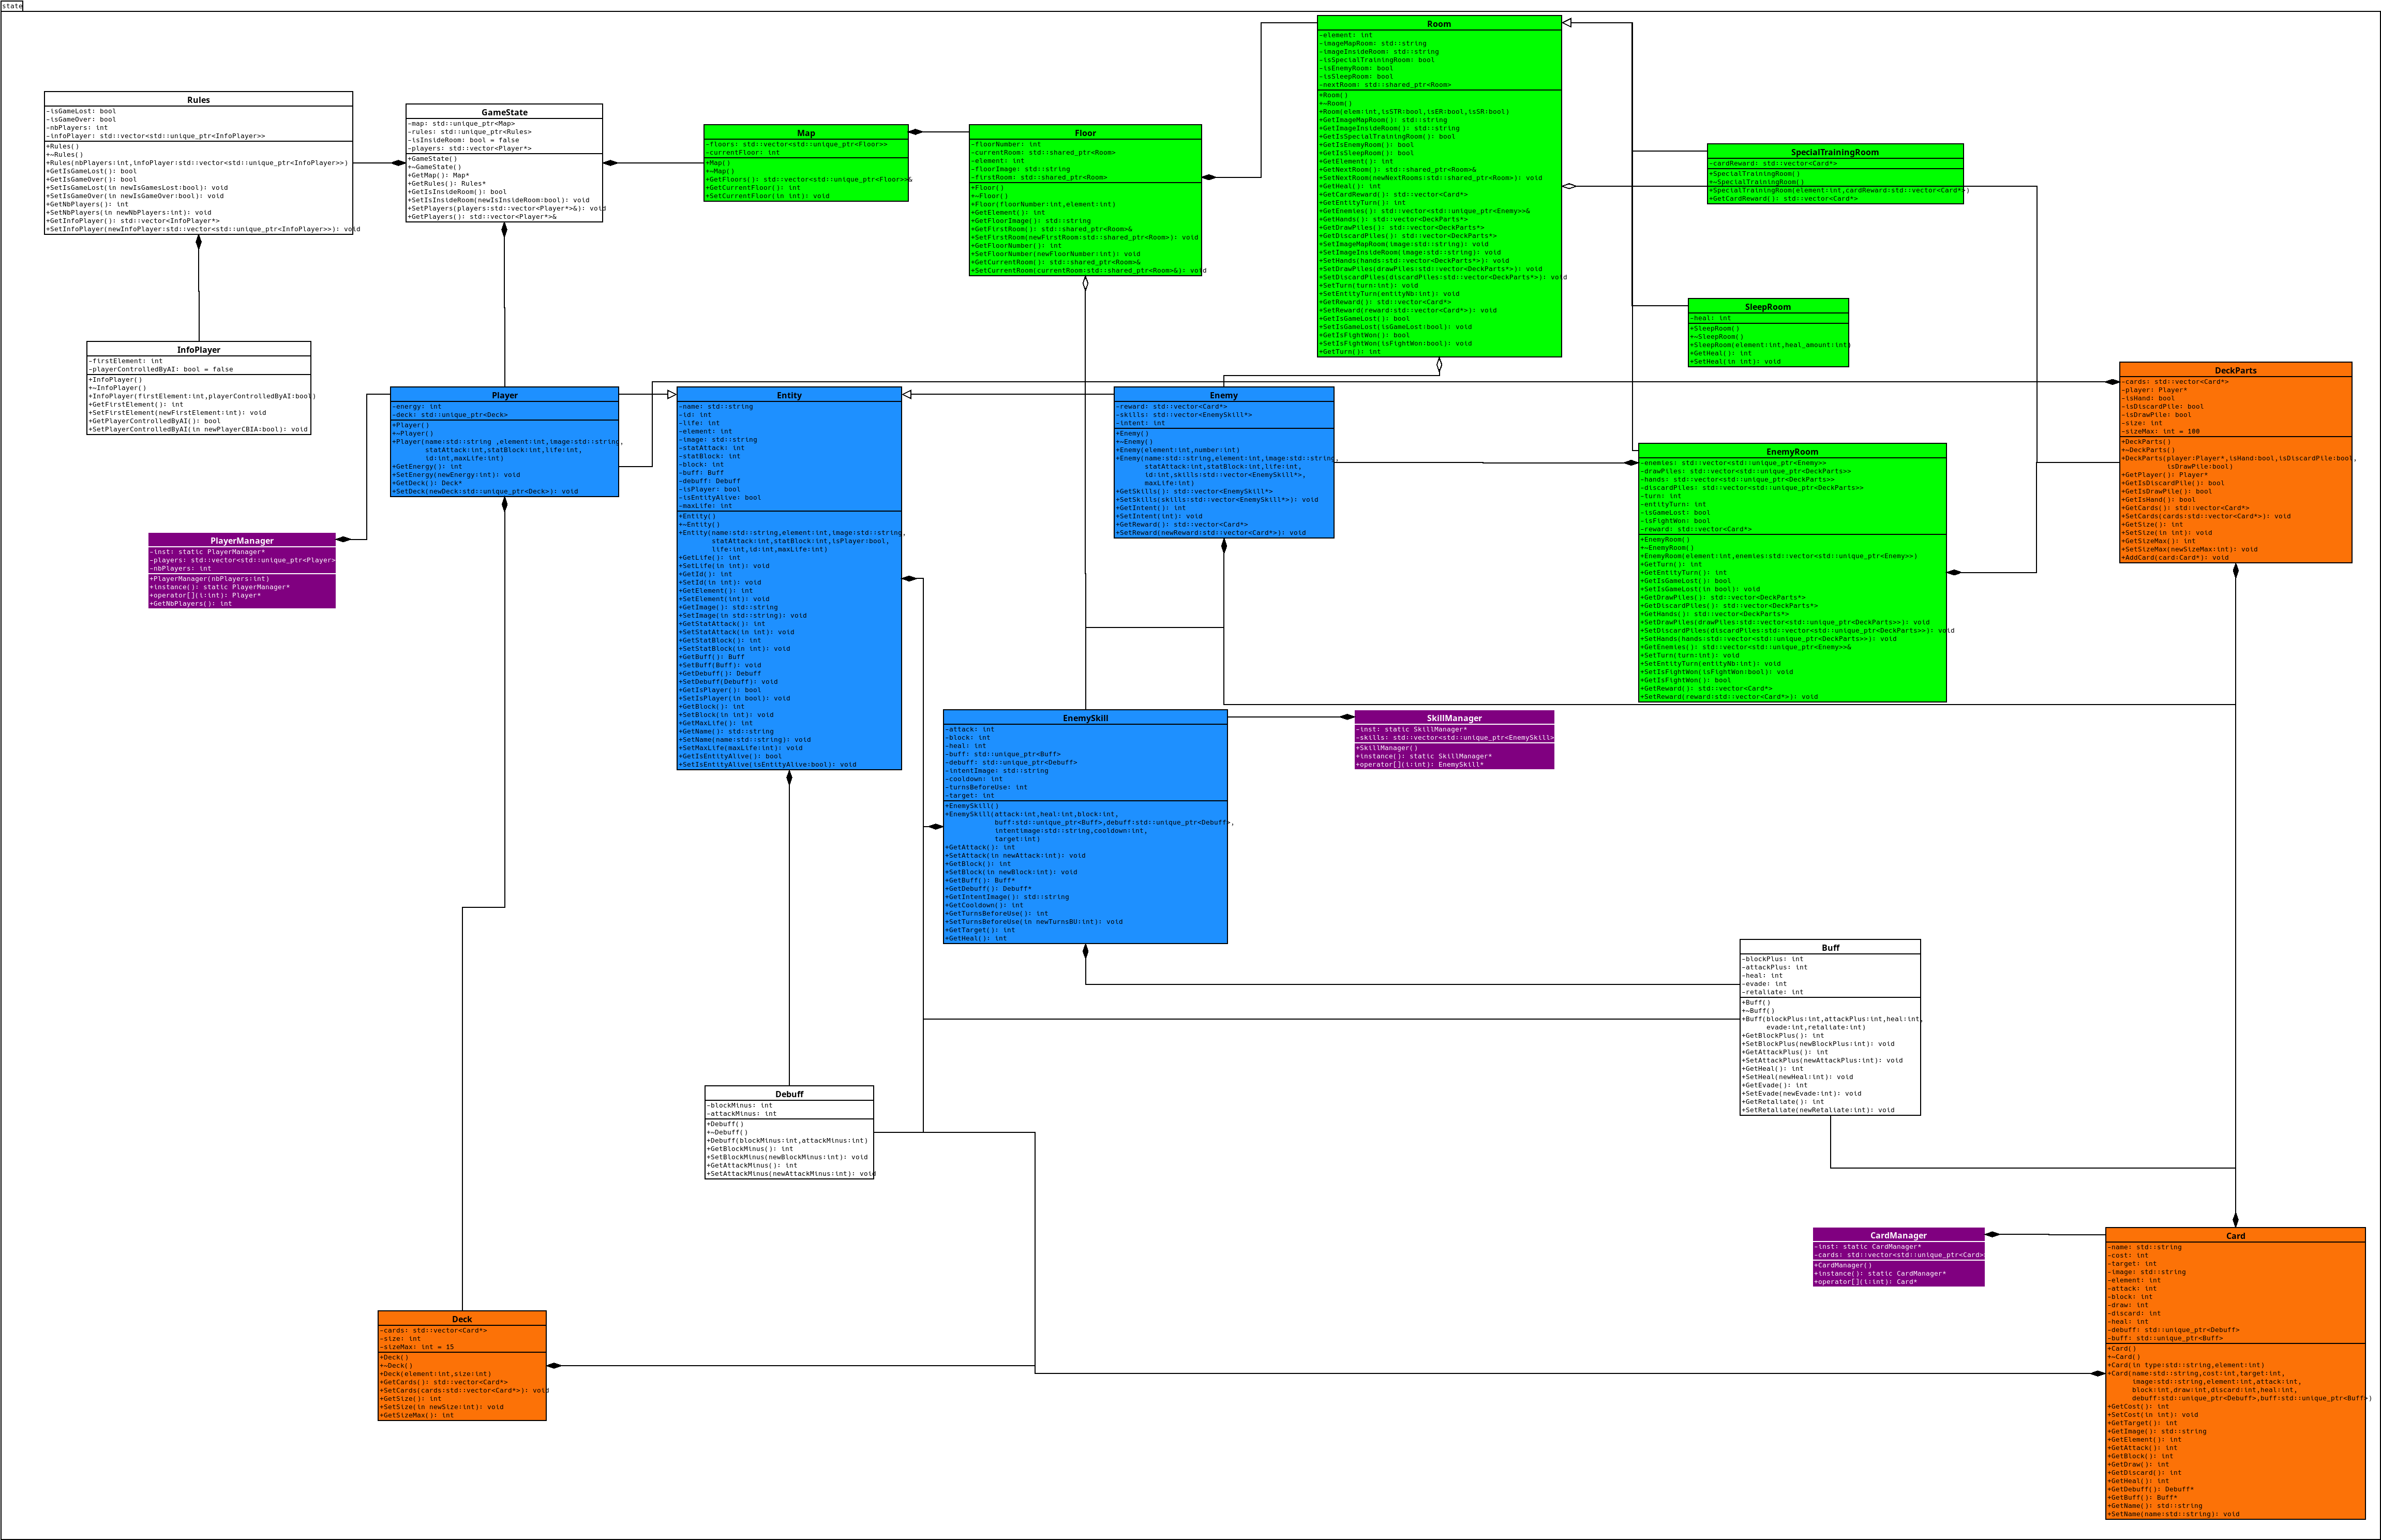
\includegraphics[width=0.8\paperheight]{images/state.png}
\caption{\label{uml:state}Diagramme des classes d'état.} 
\end{figure}
\end{landscape}

\begin{landscape}
\begin{figure}[p]
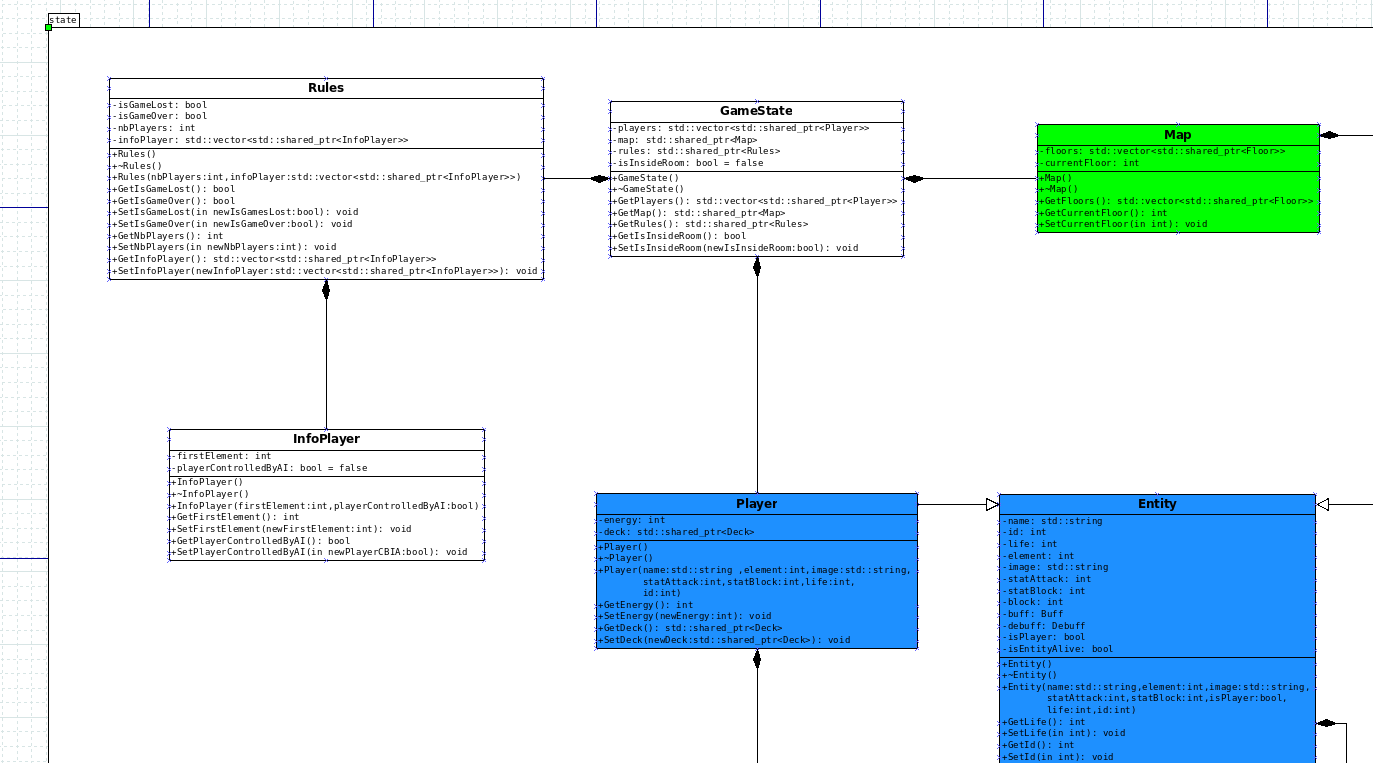
\includegraphics[width=0.8\paperheight]{images/state1.png}
\caption{\label{uml:state}Diagramme des classes d'état - état du jeu.} 
\end{figure}
\end{landscape}

\begin{landscape}
\begin{figure}[p]
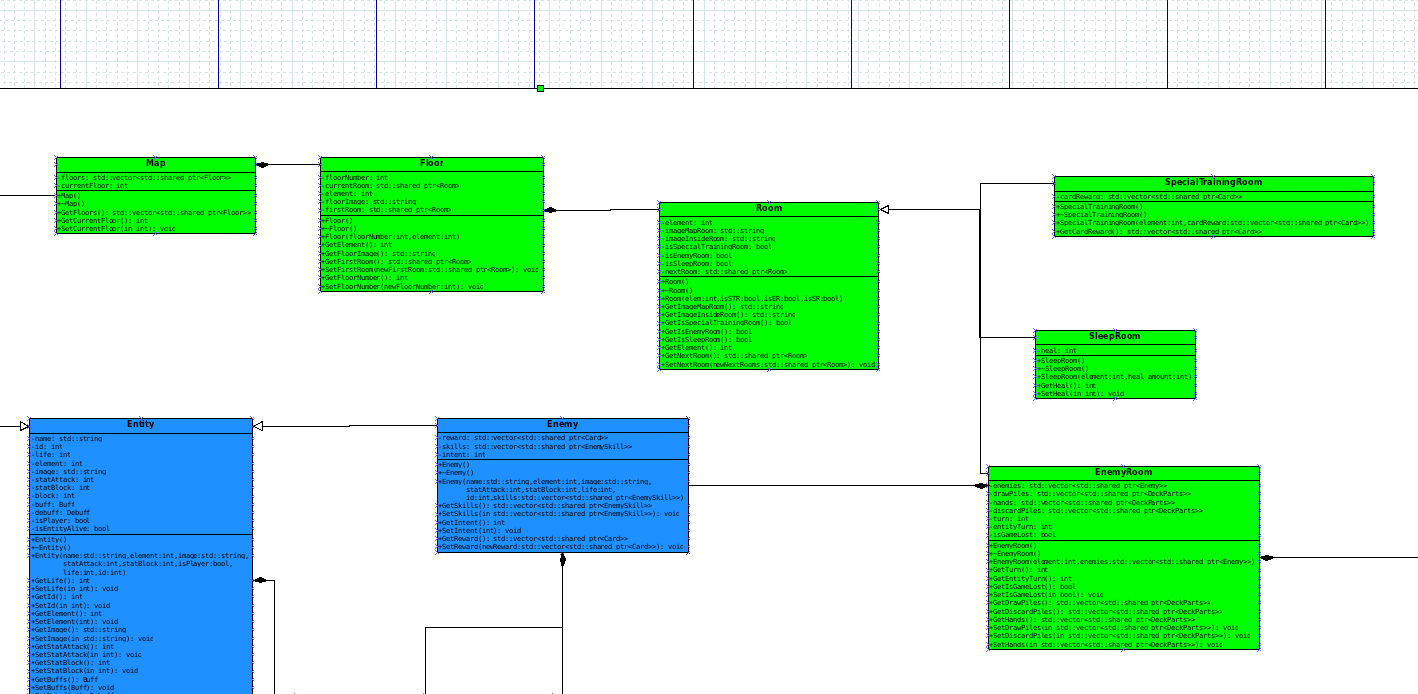
\includegraphics[width=0.8\paperheight]{images/state2.png}
\caption{\label{uml:state}Diagramme des classes d'état - état de la carte.} 
\end{figure}
\end{landscape}
\begin{landscape}
\begin{figure}[p]
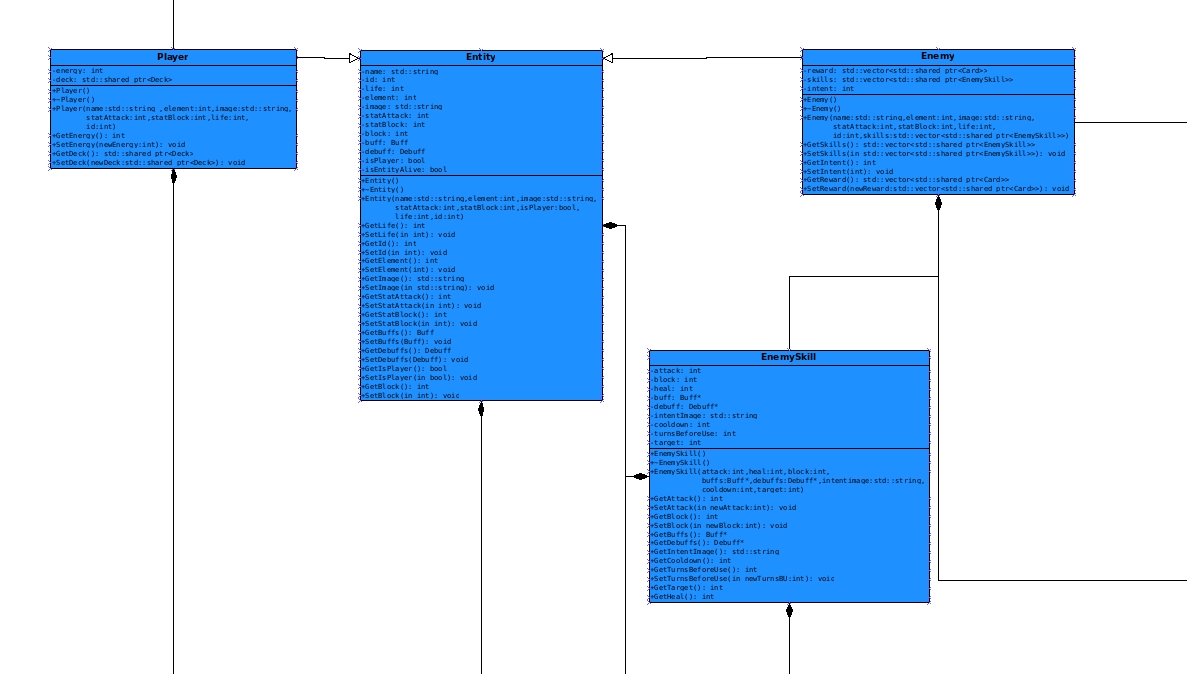
\includegraphics[width=0.8\paperheight]{images/state3.png}
\caption{\label{uml:state}Diagramme des classes d'état - état des entités.} 
\end{figure}
\end{landscape}

\begin{landscape}
\begin{figure}[p]
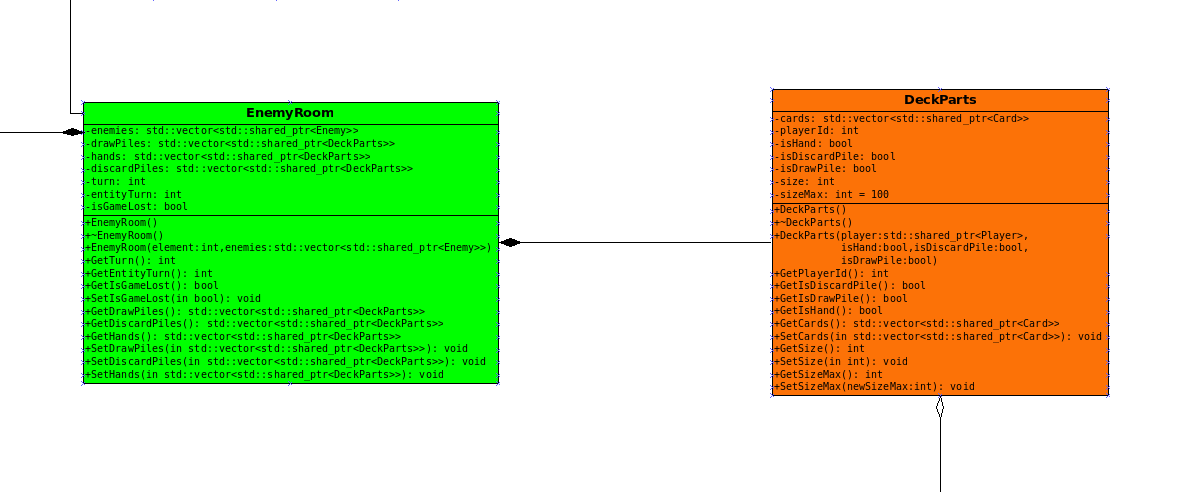
\includegraphics[width=0.8\paperheight]{images/state4.png}
\caption{\label{uml:state}Diagramme des classes d'état - état du deck 1.} 
\end{figure}
\end{landscape}

\begin{landscape}
\begin{figure}[p]
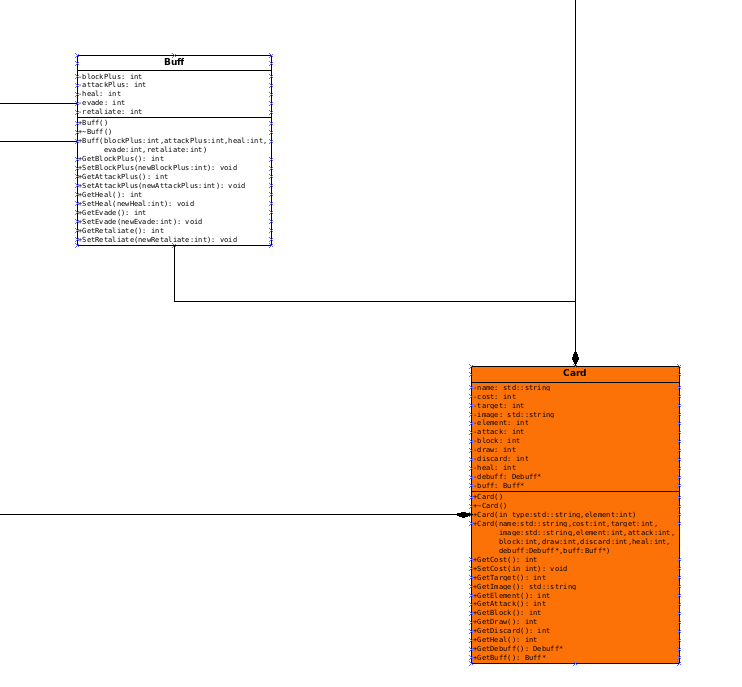
\includegraphics[width=0.5\paperheight]{images/state5.png}
\caption{\label{uml:state}Diagramme des classes d'état - état du deck 2.} 
\end{figure}
\end{landscape}

\begin{landscape}
\begin{figure}[p]
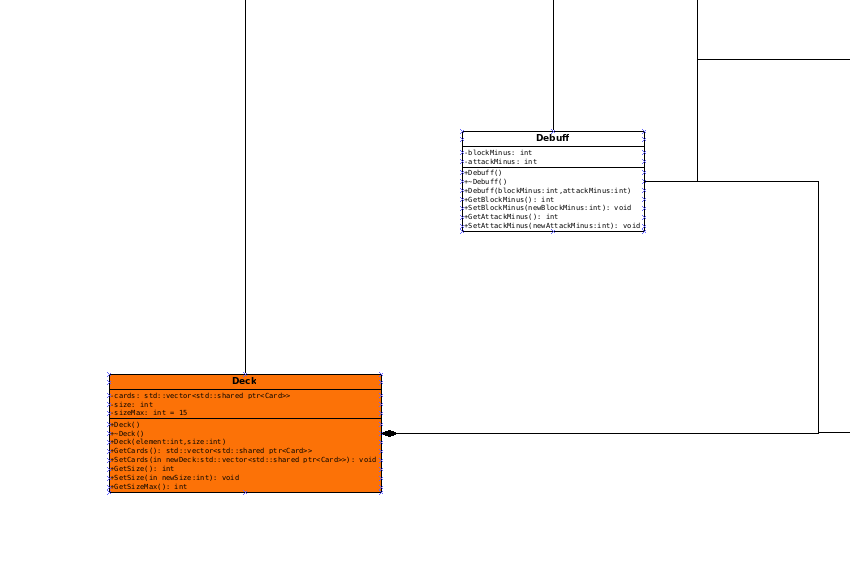
\includegraphics[width=0.8\paperheight]{images/state7.png}
\caption{\label{uml:state}Diagramme des classes d'état - état du deck 3.} 
\end{figure}
\end{landscape}


\clearpage
